\chapter{Planetbevægelse}
%
%
\section*{Planetbaner og excentricitet}
%
%
\begin{opgave}{Excentricitet og planetbaner}{1}
\opg Når $\epsilon = 0$:
\begin{align*}
	r(\phi) &= \frac{c}{1+\epsilon\cos(\phi)} = \frac{c}{1} = c \: .
\end{align*}
Afstanden er altså ens til alle vinkler. Af denne grund må den geometriske form være en cirkel, da der altid er samme afstand fra centrum til cirklen.
\opg Når $\epsilon = 1$:
\begin{align*}
	r(\phi) &= \frac{c}{1+\epsilon\cos(\phi)} = \frac{c}{1+\cos(\phi)} \: .
\end{align*}
Idet $\phi$ går mod $\pi$, da går afstanden mellem objekterne mod $\infty$:
\begin{align*}
	r(\pi) &= \frac{c}{1+\cos(\pi)} = \frac{c}{1-1} = \frac{c}{0} = \infty \: .
\end{align*}
Da banen er endelig i alle andre punkter end $\phi = \pi$, da vil der være tale om en parabelbane.
\opg For $\epsilon > 1$ vil $r(\phi) = \infty$, men dette vil ske til en vinkel $\phi < \pi$ til forskel fra tilfælde med $\epsilon = 1$. Denne vinkel vil være givet ved
\begin{align*}
	-1 &= \epsilon\cos(\phi) \Rightarrow \arccos\left(-\frac{1}{\epsilon}\right) \: .
\end{align*}
Idet funktionen for afstanden mellem de to objekter vil stige hurtigere, når $\epsilon > 1$ end når $\epsilon = 1$, da vil der være tale om en hyperbel i tilfældet $\epsilon > 1$.
\end{opgave}
%
%
\begin{opgave}{Halleys komet}{1}
\opg Fra kompendiets ligning \eqref{k-eq:r(phi)}:
\begin{align*}
	r(\phi) &= \frac{c}{1+\epsilon\cos(\phi)} \: .
\end{align*}
Idet afstanden mellem Solen og kometen er mindst, så befinder kometen sig i periapsis, hvor $\phi = 0$:
\begin{align*}
	r_{\mathrm{min}} &= \frac{c}{1+\epsilon\cos(0)}
	= \frac{c}{1+\epsilon} \: .
\end{align*}
Idet afstanden mellem Solen og kometen er størst, så befinder kometen sig i apoapsis, hvor $\phi = \pi$:
\begin{align*}
	r_{\mathrm{maks}} &= \frac{c}{1+\epsilon\cos(\pi)}
	= \frac{c}{1-\epsilon} \: .
\end{align*}
Isoleres i begge disse ligninger konstanten $c$ fås:
\begin{align*}
	r_{\mathrm{min}} &= \frac{c}{1+\epsilon} \quad \Rightarrow \quad c = r_{\mathrm{min}} (1+\epsilon) \: ,\\
	r_{\mathrm{maks}} &= \frac{c}{1-\epsilon} \quad \Rightarrow \quad c = r_{\mathrm{maks}} (1-\epsilon) \: .
\end{align*}
Da $c$ er samme konstant i de to ligninger sættes disse to lig hinanden:
\begin{align*}
	r_{\mathrm{maks}} (1-\epsilon) &= r_{\mathrm{min}} (1+\epsilon) \\
	\Rightarrow r_{\mathrm{maks}} &= \frac{1+\epsilon}{1-\epsilon} r_{\mathrm{min}} \: .
\end{align*}
%
\opg \begin{align*}
	r_{\mathrm{maks}} &= \frac{1+0,967}{1-0,967} \cdot 0,59 \, \text{AU} = \frac{1,967}{0,033} \cdot 0,59 \, \text{AU} = 35 \, \text{AU} \: .
\end{align*}
\end{opgave}
%
%
\begin{opgave}{Excentricitet}{1}
\opg I opgave \ref{opg:Halleys_komet} blev det fundet at
\begin{align*}
	r_{\mathrm{min}}(1+\epsilon) &= r_{\mathrm{maks}}(1-\epsilon) \: .
\end{align*}
Excentriciteten kan isoleres på følgende måde:
\begin{align*}
	r_{\mathrm{min}}+\epsilon r_{\mathrm{min}} &= r_{\mathrm{maks}}-\epsilon r_{\mathrm{maks}} \\
	\Rightarrow r_{\mathrm{maks}}-r_{\mathrm{min}} &= \epsilon r_{\mathrm{maks}}+\epsilon r_{\mathrm{min}}
	= (r_{\mathrm{maks}}+r_{\mathrm{min}})\epsilon \\
	\Rightarrow \epsilon &= \frac{r_{\mathrm{maks}}-r_{\mathrm{min}}}{r_{\mathrm{maks}}+r_{\mathrm{min}}} \: .
\end{align*}
%
\opg Den mindste værdi, som $\epsilon$ kan antage, er $0$, hvilket sker når $r_{\mathrm{min}} = r_{\mathrm{maks}}$.\\
Den største værdi, som $\epsilon$ kan antage, er matematisk set $1$, hvilket sker når $r_{\mathrm{min}} = 0$, men dette tilfælde giver ikke mening fysisk set, da objektet så i periapsis vil befinde sig i centrum af det objekt, som det kredser om. En anden grund til, at den største værdi af epsilon ikke kan være $1$ er, at der gøres brug af $r_{\mathrm{maks}}$, og denne værdi findes kun idet, at der er tale om en bunden bane, da objektet i en ubunden bane aldrig vil nå en maksimal afstand.\\
Idet $0 \leq \epsilon < 1$ vil der være tale om ellipsebaner.
\end{opgave}
%
%
%
\section*{Tolegemeproblemet}
%
%
\begin{opgave}{Ækvivalens i tolegemeproblemet}{1}
\begin{align*}
	R = \frac{m_\odot r + m_\oplus\cdot 0}{m_\odot + m_\oplus} =r\frac{m_\odot}{M}
\end{align*}
Hvis $r = c/(1+\epsilon\cos(\phi))$, så er $R = A/(1 + \epsilon\cos(\phi))$, hvor $A = c m_\odot/M$.
Dette betyder, at massemidtpunktet vil lave en ellipsebevægelse med samme excentricitet som Solen, men med en reduceret halv storakse (reduceret med $m_\odot/M$). Her er $\odot$ og $\oplus$ astrofysisk notation for henholdsvis Solen og Jorden.
\end{opgave}
%
%
\begin{opgave}{Ækvivalens i tolegemeproblemet II}{1}
Vi har
\begin{align*}
	R = \frac{m_\odot \cdot r_\odot + m_\oplus \cdot r_\oplus}{M} = 0
\end{align*}
og
\begin{align*}
	r = r_\oplus - r_\odot = \frac{c}{1+\epsilon\cdot\cos(\phi)}
\end{align*}
(de to er antiparallelle).
%
Så
\begin{align*}
	m_\odot \cdot r_\odot = - m_\oplus \cdot r_\oplus
\end{align*}
eller
\begin{align*}
	r_\odot = -r_\oplus \frac{m_\oplus}{m_\odot}
\end{align*}
samt
\begin{align*}
	r_\oplus = r + r_\odot
\end{align*}
%
\begin{align*}
	r_\odot &= - \frac{m_\oplus}{m_\odot} (r + r_\odot) \\
r_\odot \left(1 + \frac{m_\oplus}{m_\odot}\right) &= - \frac{m_\oplus}{m_\odot} r \\
r_\odot &= - \frac{m_\oplus}{m_\odot + m_\oplus} r \\
        &= - \frac{m_\oplus}{M} r
\end{align*}
%
Tilsvarende for Jorden:
\begin{align*}
	r_\oplus &= - \frac{m_\odot}{m_\oplus} r_\odot \\
	r_\odot &= r_\oplus - r \\[5mm]
	r_\oplus &= - \frac{m_\odot}{m_\oplus} (r_\oplus - r) \\
	r_\oplus \left(1 + \frac{m_\odot}{m_\oplus}\right) &=  \frac{m_\odot}{m_\oplus} r \\
	r_\oplus &= \frac{m_\odot}{M} r
\end{align*}
\end{opgave}
%
%
%
\section*{Bevægelsesligningerne}
%
%
\begin{figure}
	\centering
	\begin{subfigure}{0.49\textwidth}
		\centering
		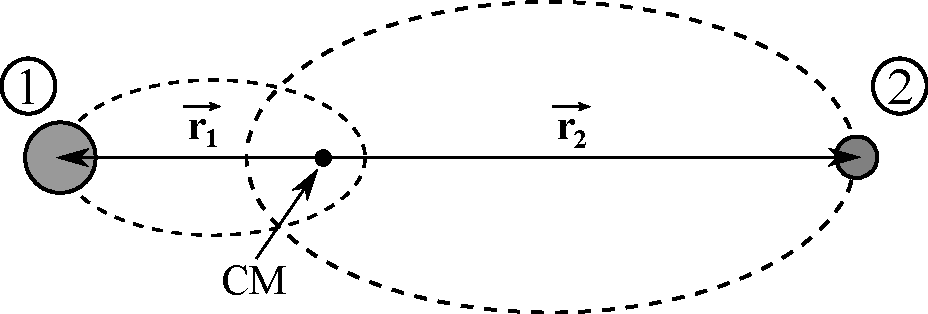
\includegraphics[width=0.95\textwidth]{Planetbevaegelse/Bevarelse_af_impulsmoment_spg1}
		\caption{Spørgsmål 1.}
		\label{fig:Bevarelse_af_impulsmoment_spg1}
	\end{subfigure}
	\hfill
	\vspace{5mm}
	\begin{subfigure}{0.49\textwidth}
		\centering
		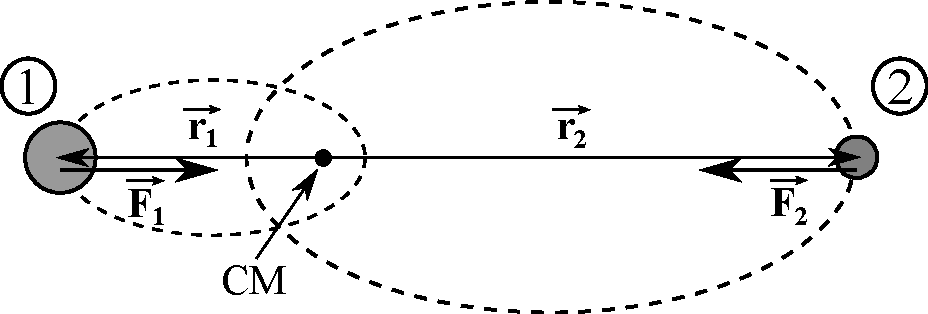
\includegraphics[width=0.95\textwidth]{Planetbevaegelse/Bevarelse_af_impulsmoment_spg2}
		\caption{Spørgsmål 2.}
		\label{fig:Bevarelse_af_impulsmoment_spg2}
	\end{subfigure}
	\begin{subfigure}{0.70\textwidth}
		\centering
		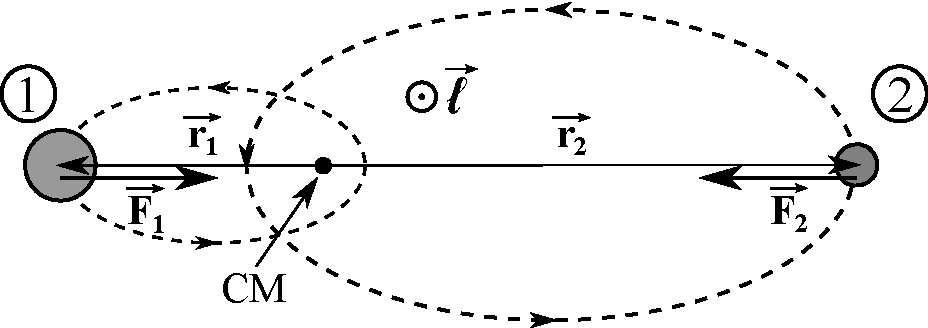
\includegraphics[width=0.95\textwidth]{Planetbevaegelse/Bevarelse_af_impulsmoment_spg5}
		\caption{Spørgsmål 5.}
		\label{fig:Bevarelse_af_impulsmoment_spg5}
	\end{subfigure}
	\caption{Grafiske besvarelser til opgave \ref{opg:Bevarelse_af_impulsmoment}. Kræfterne er på disse tegning tegnet lidt under massemidtpunktet af hvert legeme for at gøre figuren mere overskuelig.}
	\label{fig:Bevarelse_af_impulsmoment}
\end{figure}
%
\begin{opgave}{Bevarelse af impulsmoment}{1}
\opg Se figur \ref{fig:Bevarelse_af_impulsmoment_spg1}.\\
Banernes excentricitet skal være ens, mens banernes halve storakse blot er skaleret efter forholdet mellem de to legemers afstande til massemidtpunktet.
%
\opg Se figur \ref{fig:Bevarelse_af_impulsmoment_spg2}.\\
Ifølge Newtons 3. lov skal de to kræfter være lige store og modsatrettede.
%
\opg Kraftmomentet er givet ved
\begin{align*}
	\v{\tau} &= \v{r} \times \v{F} \: ,
\end{align*}
men siden det for begge legemer gør sig gældende, at $\v{r}_i \parallel \v{F}_i \: , \: \forall \, i = 1,2$, da vil krydsproduktet mellem disse to vektorer give $0$, hvorfor
\begin{align*}
	\v{\tau}_i = \v{0} \: , \enspace \forall \, i = 1,2 \: .
\end{align*}
%
\opg Af kompendiets ligning \eqref{k-eq:sum_tau_lig_aflede_impulsmoment} vides det at
\begin{align*}
	\v{\tau}_i &= \dif{t}{\v{\ell}_i} \: ,
\end{align*}
og siden det blev fundet, at $\v{\tau}_i = \v{0}$, da betyder det, at den tidsafledede af impulsmomentet er $\v{0}$, hvilket gør sig gældende, hvis impulsmomenter er konstant.\\
Idet at hvert af impulsmomenterne er konstant, da vil det også betyde, at det totale impulsmoment er konstant.
%
\opg Se figur \ref{fig:Bevarelse_af_impulsmoment_spg5}.\\
Impulsmomentet er givet ved
\begin{align*}
	\v{\ell} &= \v{r} \times \v{p} \: ,
\end{align*}
hvortil højrehåndsreglen benyttes til at finde retningen af hvert af impulsmomenterne, da retningen af  afstandsvektoren $\v{r}$ og hastigheden $\v{v}$, og dermed impulsen $\v{p}$, kendes. Retningen af de to impulsmomenter vil være den samme, hvorfor det totale impulsmoment også vil gå i denne retning.
\end{opgave}
%
%
\begin{opgave}{Keplers 3. lov}{2}
\opg Vi ved at
\begin{align*}
	P &= \frac{A}{\d A / \d t}
	= \frac{\pi a b}{\left(\dfrac{\ell}{2\mu}\right)} \\
	\Rightarrow	P^2 &= \frac{4 \pi^2 a^2 b^2 \mu^2}{\ell^2} \: .
\end{align*}
Fra kompendiets ligning \eqref{k-eq:Planetbevaegelse_a_b_og_d} vides det at
\begin{align*}
	a &= \frac{c}{1-\epsilon^2} \, \\
	b &= \frac{c}{\sqrt{1-\epsilon^2}} \: ,
\end{align*}
og udtrykkes $b^2$ ved $a^2$ bliver det
\begin{align*}
	b^2 &= a^2 \frac{(1-\epsilon^2)^2}{1-\epsilon^2}
	= a^2 (1-\epsilon^2) \: ,
\end{align*}
hvilket kan indsættes i udtrykket for $P^2$:
\begin{align*}
	P^2 &= \frac{4 \pi^2 a^2 a^2 (1-\epsilon^2) \mu^2}{\ell^2}
	= \frac{4 \pi^2 a^4 (1-\epsilon^2) \mu^2}{\ell^2} \: .
\end{align*}
Hernæst vides det fra kompendiet, at
\begin{align*}
	c &= \frac{\ell^2}{Gm_1m_2\mu} \\
	\Rightarrow \ell^2 &= Gm_1m_2\mu c \: ,
\end{align*}
hvorfor $P^2$ bliver
\begin{align*}
	P^2 &= \frac{4 \pi^2 a^4 (1-\epsilon^2) \mu^2}{Gm_1m_2\mu c}
	= \frac{4 \pi^2 a^4 (1-\epsilon^2) \mu}{Gm_1m_2 c} \: .
\end{align*}
Hernæst indsættes et udtryk for $c$ fået fra ligningen for $a$,
\begin{align*}
	c &= a(1-\epsilon^2) \: ,
\end{align*}
i udtrykket for $P^2$
\begin{align*}
	P^2 &= \frac{4 \pi^2 a^4 (1-\epsilon^2) \mu}{Gm_1m_2 a(1-\epsilon^2)}
	= \frac{4 \pi^2 a^3 \mu}{Gm_1m_2} \: .
\end{align*}
Sidst indsættes udtrykket for den reducerede masse,
\begin{align*}
	\mu &= \frac{m_1m_2}{m_1+m_2} \: ,
\end{align*}
i $P^2$:
\begin{align*}
	P^2 &= \frac{4 \pi^2 a^4 (1-\epsilon^2) \dfrac{m_1m_2}{m_1+m_2}}{Gm_1m_2 a(1-\epsilon^2)}
	= \frac{4 \pi^2}{G(m_1+m_2)}a^3 \: .
\end{align*}
\end{opgave}
%
%
\begin{opgave}{Energibevarelse og excentricitet}{3}
\opg Hastigheden skifter fortegn, når kometen passerer $r_{\mathrm{min}}$. Derved må $v(r_{\mathrm{min}}) = 0$. Af dette bliver energien i $r_{\mathrm{min}}$:
\begin{align*}
	E(r_{\mathrm{min}}) &= V_{eff}(r_{\mathrm{min}})
	= \frac{\ell^2}{2\mu r_{\mathrm{min}}^2} - \frac{\gamma}{r_{\mathrm{min}}}
	= \frac{1}{2 r_{\mathrm{min}}} \left(\frac{\ell^2}{\mu r_{\mathrm{min}}} - 2\gamma\right) \: .
\end{align*}
%
\opg Fra kompendiets ligning \eqref{k-eq:r(phi)} har vi, at
\begin{align*}
	r &= \frac{c}{1+\epsilon\cos(\phi)} \: ,
\end{align*}
hvilket for $r_{\mathrm{min}}$ bliver
\begin{align*}
	r_{\mathrm{min}} &= \frac{c}{1+\epsilon\cos(0)}
	= \frac{c}{1+\epsilon} \: .
\end{align*}
Ved at indsætte den givne værdi for $c$ fås
\begin{align*}
	r_{\mathrm{min}} &= \frac{\ell^2}{\gamma\mu(1+\epsilon)} \: .
\end{align*}
%
\opg Her indsættes resultatet fra spørgsmål 2 i resultatet fra spørgsmål 1:
\begin{align*}
	E = \frac{\gamma\mu(1+\epsilon)}{2 \ell^2} \left(\gamma(1+\epsilon) - 2\gamma\right)
	= \frac{\gamma^2\mu}{2\ell^2} (\epsilon+1)(\epsilon-1)
	= (\epsilon^2-1)\frac{\gamma^2\mu}{2\ell^2} \: .
\end{align*}
Da der er energibevarelse må denne energi være den samme, som den til en vilkårligt andet tidspunkt eller sted i banen.
%
\opg Hvis energien skal være negativ kræves, at $\epsilon^2 < 1$, altså $0\leq \epsilon < 1$. Dette er excentriciteten for en ellipsebane (eller cirkelbane hvis $\epsilon = 0$), hvilket stemmer fint overens med at kometen er i en bunden bane, når den potentielle energi er større end den kinetiske.\\
Hvis energien er $0$ kræves, at $\epsilon^2 = 1$, altså $\epsilon = 1$. Dette er svarende en parabelbane, hvor kometen netop undslipper, men dette sker så langsomt som muligt, da den kinetiske energi netop opvejer den potentielle energi.\\
Hvis energien er positiv, da må $\epsilon^2 > 1$, altså $\epsilon > 1$, hvorfor der må være tale om en hyperbelbane.
\end{opgave}
%
%
%
\section*{Baneskift}
%
%
\begin{figure}
	\centering
	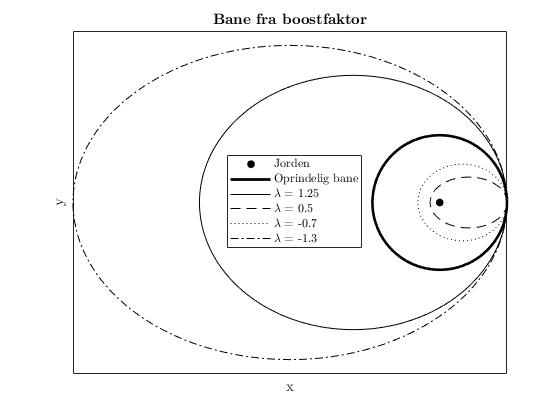
\includegraphics[width=0.85\textwidth]{Planetbevaegelse/Boostfaktor_tegninger.png}
	\caption{Baner fundet fra forskellige boostfaktorer.}
	\label{fig:Boostfaktor_tegninger}
\end{figure}
%
\begin{opgave}{Boostfaktor}{1}
Se figur \ref{fig:Boostfaktor_tegninger}. Her er forskellige værdier af de positive og negative boostfaktorer valgt, da fortegnet for boostfaktoren blot vender bevægelsesretningen.
\end{opgave}
%
%
\begin{opgave}{Boostkraft}{2}
\opg \begin{align*}
	\v{F} &= m\v{a}
	\xleq{\v{a} = \dif{t}{\v{v}}}
	m \dif{t}{\v{v}}
	= \dif{t}{m\v{v}}
	\xleq{\v{p} = m\v{a}}
	\dif{t}{\v{p}}
	= \lim\limits_{t \rightarrow 0} \frac{\Delta \v{p}}{\Delta t} \: .
\end{align*}
\opg Først finds impulsmomentet i $P$ før og efter boostet, hhv. $\ell_1$ og $\ell_2$:
\begin{align*}
	\ell_1 &= mv_1r_1 \: , \\
	\ell_2 &= mv_2r_2
	\xleq{\lambda = \frac{v_2}{v_1}}
	m \lambda v_1 r_2 \: ,
\end{align*}
hvor $m$ er satellittens masse, som antages ikke at ændre sig under boostet, $v$ er hastigheden og $r$ er afstanden mellem Jorden og satellitten.
Forskellen i impulsmoment findes:
\begin{align*}
	\Delta \ell &= \ell_2 - \ell_1
	= m \lambda v_1 r_2 - mv_1r_1
	\xleq{r_1(P) = r_2(P)}
	mv_1r_1(\lambda - 1) \: ,
\end{align*}
Da impulsmomentet findes som
\begin{align*}
	\ell &= rp \: ,
\end{align*}
så bliver ovenstående
\begin{align*}
	\Delta \ell &= r_1 \Delta p \: ,
\end{align*}
hvor
\begin{align*}
	\Delta p = mv_1(\lambda-1) \: .
\end{align*}
Boostkraften bliver dermed
\begin{align*}
	F_{av} &= \frac{\Delta p}{\Delta t}
	= \frac{mv_1}{\Delta t} (\lambda-1) \: .
\end{align*}
\end{opgave}
%
%
\begin{opgave}{Hohmannbane}{2}
\opg Hohmannbanen har apsis i de to baner med radius hhv. $R_1$ og $R_3 = 2R_1$. Da $R_3 > R_1$, må Hohmannbanen havde apoapsis i $P'$ og periapsis i $P$.
%
\opg Da bane 1 er cirkulær, så vil excentriciteten af denne bane være $\epsilon_1 = 0$. Ved brug af kompendiets ligning \eqref{k-eq:Generel_formel_r(phi)} kan det ses, at $R_1 = c_1$:
\begin{align*}
	R_1 &= \frac{c_1}{1+\epsilon_1\cos(\phi-\delta)}
	\xleq{\epsilon_1 = 0}
	\frac{c_1}{1} = c_1 \: .
\end{align*}
Excentriciteten af Hohmannbanen kan nu findes ved kompendiets ligning \eqref{k-eq:Baneskift_epsilon2}:
\begin{align*}
	\epsilon_2 &= \lambda^2\epsilon_1+(\lambda^2-1)
	\xleq{\epsilon_1 = 0}
	\lambda^2-1 \: .
\end{align*}
Idet satelitten er i apoapsis i Hohmannbanen ($P'$) skal $r_2(P') = R_3$. Der gøres her igen brug af kompendiets ligning \eqref{k-eq:Generel_formel_r(phi)}:
\begin{align*}
	R_3 &= r_2(P') = \frac{c_2}{1+\epsilon_2\cos(\pi)} = \frac{c_2}{1-\epsilon_2}
	\xleq{\epsilon_2 = \lambda^2-1}
	\frac{c_2}{1-(\lambda^2-1)} = \frac{c_2}{2-\lambda^2} \: .
\end{align*}
$c_2$ kan ved kompendiets ligning \eqref{k-eq:Baneskift_c2}:
\begin{align*}
	c_2 &= \lambda^2 c_1
	\xleq{c_1 = R_1}
	\lambda^2 R_1 \: .
\end{align*}
Indsættes dette i udtrykket for $R_3$ fra tidligere fås:
\begin{align*}
	R_3 &= \frac{\lambda^2 R_1}{2-\lambda^2} \\
	\Rightarrow \frac{R_1}{R_3} &= \frac{2-\lambda^2}{\lambda^2} = \frac{2}{\lambda^2} - 1 \\
	\Rightarrow \frac{2}{\lambda^2} &= \frac{R_1}{R_3} + 1 = \frac{R_1+R_3}{R_3} \\
	\Rightarrow \lambda^2 &= \frac{2R_3}{R_1+R_3} \\
	\Rightarrow \lambda &= \sqrt{\frac{2R_3}{R_1+R_3}}
	\xleq{R_3 = 2R_1}
	\sqrt{\frac{2 \cdot 2R_1}{R_1+2R_1}} = \sqrt{\frac{4R_1}{3R_1}} = \sqrt{\frac{4}{3}} \: .
\end{align*}
Altså vil boostfaktoren i punktet $P$ være $\lambda = \sqrt{4/3}$.
%
\opg Da bane 1 er cirkulær, så vil excentriciteten af denne bane være $\epsilon_3 = 0$. Ved brug af kompendiets ligning \eqref{k-eq:Generel_formel_r(phi)} kan det ses, at $R_3 = c_3$:
\begin{align*}
	R_3 &= \frac{c_3}{1+\epsilon_3\cos(\phi-\delta)}
	\xleq{\epsilon_3 = 0}
	\frac{c_3}{1} = c_3 \: .
\end{align*}
$c_3$ kan nu beskrives ved kompendiets ligning \eqref{k-eq:Baneskift_c2}:
\begin{align*}
	c_3 &= \lambda'^2 c_2
	\xleq{c_2 = \lambda^2 c_1}
	\lambda'^2 \lambda^2 c_1
	\xleq{c_1 = R_1}
	\lambda'^2 \lambda^2 R_1 \: .
\end{align*}
Heri isoleres nu for at finde $\lambda'$:
\begin{align*}
	\lambda'^2 &= \frac{c_3}{\lambda^2 R_1}
	\xleq{c_3 = R_3}
	\frac{R_3}{\lambda^2 R_1}
	\xleq{\lambda = \sqrt{\frac{2R_3}{R_1+R_3}}}
	\frac{R_3}{\dfrac{2R_3}{R_1+R_3} R_1}
	= \frac{R_3}{\left(\dfrac{2R_1R_3}{R_1+R_3}\right)}
	= R_3 \frac{R_1+R_3}{2R_1R_3}
	= \frac{R_1+R_3}{2R_1} \\
	\lambda' &= \sqrt{\frac{R_1+R_3}{2R_1}}
	\xleq{R_3 = 2R_1}
	\sqrt{\frac{R_1+2R_1}{2R_1}}
	= \sqrt{\frac{3R_1}{2R_1}}
	= \sqrt{\frac{3}{2}} \: .
\end{align*}
Altså vil boostfaktoren i punktet $P'$ være $\lambda' = \sqrt{3/2}$.
%
\opg Da der er impulsmomentbevarelse, da vil følgende gøre sig gældende for Hohmannbanen:
\begin{align*}
	m v_2(P)r_2(P) &= m v_2(P')r_2(P') \: ,
\end{align*}
hvor $m$ er satellittens masse, som antages konstant under hele baneskiftet, hvorfor denne går ud.\\
Herudover vides det, at $r_2(P) = R_1$ og $r_2(P') = R_3$, hvorfor ligningen bliver
\begin{align*}
	v_2(P)R_1 &= v_2(P')R_3 \: .
\end{align*}
Af formlen for boostfaktoren, kompendiets ligning \eqref{k-eq:Baneskift_boostfaktor}, fås
\begin{align*}
	\begin{aligned}
		\lambda &= \frac{v_2(P)}{v_1(P)} \\
		&\Downarrow \\
		v_2(P) &= \lambda v_1
	\end{aligned}
	\qquad \qquad
	\begin{aligned}
		\lambda' &= \frac{v_3(P')}{v_2(P')} \\
		&\Downarrow \\
		v_2(P') &= \frac{v_3}{\lambda'}
	\end{aligned}
\end{align*}
hvilket indsættes i ligningen ovenfor:
\begin{align*}
	\lambda v_1 R_1 &= \frac{v_3}{\lambda'} R_3 \: ,
\end{align*}
og $v_3$ isoleres
\begin{align*}
	v_3 &= \frac{\lambda' \lambda v_1 R_1}{R_3}
	= \sqrt{\frac{3}{2}} \sqrt{\frac{4}{3}}\frac{v_1 R_1}{R_3}
	= \sqrt{\frac{12}{6}} \frac{v_1 R_1}{R_3}
	\xleq{R_3 = 2R_1}
	\sqrt{2} \frac{v_1 R_1}{2R_1}
	\xleq{\frac{\sqrt{2}}{2} = \frac{1}{\sqrt{2}}}
	\frac{1}{\sqrt{2}} v_1 \: .
\end{align*}
Altså er hastigheden af satellitten i den nye bane udtrykt ved hastigheden i begyndelsesbanen $v_3 = v_1/\sqrt{2}$.
\end{opgave}
%
%
\begin{opgave}{Hohmannbane II}{2}
Fra opgave \ref{opg:Hohmannbane} blev det fundet, at boostfaktoren for et skift mellem fra en startbane til en Hohmannbane er givet ved
\begin{align} \label{eq:Boostfaktor_generel}
	\lambda &= \sqrt{\frac{2R_{\text{efter}}}{R_{før}+R_{\text{efter}}}} \: ,
\end{align}
og boostfaktoren for et skift mellem Hohmannbanen og slutbanen er givet ved
\begin{align} \label{eq:Boostfaktor_maerke_generel}
	\lambda' &= \sqrt{\frac{R_{\text{før}}+R_{\text{efter}}}{2R_{\text{før}}}} \: ,
\end{align}
hvor $R_{\text{før}}$ er radius af den første bane, altså banen inden skiftet til Hohmannbanen, og $R_{\text{efter}}$ er radius af den sidste bane, altså banen der kommer af skiftet fra Hohmannbanen.
%
\opg Der er tale om et skift fra en cirkulær bane (A) til en Hohmannbane (1), hvorfor ligning \eqref{eq:Boostfaktor_generel} bruges. Her er $R_{\text{før}} = R_A$ og $R_{\text{efter}} = R_C = (9/2)R_A$:
\begin{align*}
	\lambda_1 &= \sqrt{\frac{2\cdot \dfrac{9}{2}R_A}{R_A+\dfrac{9}{2}R_A}}
	= \sqrt{\frac{9R_A}{\dfrac{11}{2}R_A}}
	= \sqrt{\frac{18R_A}{11R_A}}
	= \sqrt{\frac{18}{11}} \: .
\end{align*}
%
\opg Der er tale om et skift fra en Hohmannbane (1) til en cirkulær bane (C), hvorfor ligning \eqref{eq:Boostfaktor_maerke_generel} bruges. Her er $R_{\text{før}} = R_A$ og $R_{\text{efter}} = R_C = (9/2)R_A$:
\begin{align*}
	\lambda_1' &= \sqrt{\frac{R_A+\dfrac{9}{2}R_A}{2R_A}}
	= \sqrt{\frac{\dfrac{11}{2}R_A}{2R_A}}
	= \sqrt{\frac{11}{4}\frac{R_A}{R_A}}
	= \sqrt{\frac{11}{4}} \: .
\end{align*}
%
\opg Der er tale om et skift fra en cirkulær bane (C) til en Hohmannbane (2), hvorfor ligning \eqref{eq:Boostfaktor_generel} bruges. Her er $R_{\text{før}} = R_C = (3/2)R_B$ og $R_{\text{efter}} = R_B$:
\begin{align*}
	\lambda_2 &= \sqrt{\frac{2R_B}{\dfrac{3}{2}R_B+R_B}}
	= \sqrt{\frac{2R_B}{\dfrac{5}{2}R_B}}
	= \sqrt{\frac{4R_B}{5R_B}}
	= \sqrt{\frac{4}{5}} \: .
\end{align*}
\opg Der er tale om et skift fra en Hohmannbane (2) til en cirkulær bane (B), hvorfor ligning \eqref{eq:Boostfaktor_maerke_generel} bruges. Her er $R_{\text{før}} = R_C = (3/2)R_B$ og $R_{\text{efter}} = R_B$:
\begin{align*}
	\lambda_2' &= \sqrt{\frac{\dfrac{3}{2}R_B+R_B}{2\cdot\dfrac{3}{2}R_B}}
	= \sqrt{\frac{\dfrac{5}{2}R_B}{3R_B}}
	= \sqrt{\frac{5}{6}\frac{R_B}{R_B}}
	= \sqrt{\frac{5}{6}} \: .
\end{align*}
%
\opg Boostfaktorerne $\lambda_1$ og $\lambda_2$ er på samme form, formen fra ligning \eqref{eq:Boostfaktor_generel}, mens boostfaktorerne $\lambda_1'$ og $\lambda_2'$ er på samme form, formen fra ligning \eqref{eq:Boostfaktor_maerke_generel}.
\end{opgave}